% Options for packages loaded elsewhere
\PassOptionsToPackage{unicode}{hyperref}
\PassOptionsToPackage{hyphens}{url}
%
\documentclass[
]{article}
\usepackage{lmodern}
\usepackage{amsmath}
\usepackage{ifxetex,ifluatex}

\bibliographystyle{plain}
\usepackage{url}
\usepackage{hyperref}
\ifnum 0\ifxetex 1\fi\ifluatex 1\fi=0 % if pdftex
  \usepackage[T1]{fontenc}
  \usepackage[utf8]{inputenc}
  \usepackage{textcomp} % provide euro and other symbols
  \usepackage{amssymb}
\else % if luatex or xetex
  \usepackage{unicode-math}
  \defaultfontfeatures{Scale=MatchLowercase}
  \defaultfontfeatures[\rmfamily]{Ligatures=TeX,Scale=1}
\fi
% Use upquote if available, for straight quotes in verbatim environments
\IfFileExists{upquote.sty}{\usepackage{upquote}}{}
\IfFileExists{microtype.sty}{% use microtype if available
  \usepackage[]{microtype}
  \UseMicrotypeSet[protrusion]{basicmath} % disable protrusion for tt fonts
}{}
\makeatletter
\@ifundefined{KOMAClassName}{% if non-KOMA class
  \IfFileExists{parskip.sty}{%
    \usepackage{parskip}
  }{% else
    \setlength{\parindent}{0pt}
    \setlength{\parskip}{6pt plus 2pt minus 1pt}}
}{% if KOMA class
  \KOMAoptions{parskip=half}}
\makeatother
\usepackage{xcolor}
\IfFileExists{xurl.sty}{\usepackage{xurl}}{} % add URL line breaks if available
\IfFileExists{bookmark.sty}{\usepackage{bookmark}}{\usepackage{hyperref}}
\hypersetup{
  pdftitle={Under kølerhjelmen på Kafka og RabbitMQ},
  hidelinks,
  pdfcreator={LaTeX via pandoc}}
\urlstyle{same} % disable monospaced font for URLs
\usepackage{longtable,booktabs}
\usepackage{calc} % for calculating minipage widths
% Correct order of tables after \paragraph or \subparagraph
\usepackage{etoolbox}
\makeatletter
\patchcmd\longtable{\par}{\if@noskipsec\mbox{}\fi\par}{}{}
\makeatother
% Allow footnotes in longtable head/foot
\IfFileExists{footnotehyper.sty}{\usepackage{footnotehyper}}{\usepackage{footnote}}
\makesavenoteenv{longtable}
\usepackage{graphicx}
\makeatletter
\def\maxwidth{\ifdim\Gin@nat@width>\linewidth\linewidth\else\Gin@nat@width\fi}
\def\maxheight{\ifdim\Gin@nat@height>\textheight\textheight\else\Gin@nat@height\fi}
\makeatother
% Scale images if necessary, so that they will not overflow the page
% margins by default, and it is still possible to overwrite the defaults
% using explicit options in \includegraphics[width, height, ...]{}
\setkeys{Gin}{width=\maxwidth,height=\maxheight,keepaspectratio}
% Set default figure placement to htbp
\makeatletter
\def\fps@figure{htbp}
\makeatother
\setlength{\emergencystretch}{3em} % prevent overfull lines
\providecommand{\tightlist}{%
  \setlength{\itemsep}{0pt}\setlength{\parskip}{0pt}}
\setcounter{secnumdepth}{-\maxdimen} % remove section numbering
\ifluatex
  \usepackage{selnolig}  % disable illegal ligatures
\fi

\title{Under kølerhjelmen på Kafka og RabbitMQ}
\author{Adam Saidane, Emil Valbak Hermansen, Sebastian Lundsgaard-Larsen}
\date{11-12-2020}


\begin{document}
\maketitle
\textit{When you need to send data between applications or microservices it can be difficult to choose the right technology. Two of these are Kafka and RabbitMQ, but when are they the right match for the job? We will uncover their individual advantages and shortcomings and show benchmarks of which technology is faster. After reading this article you will find out that RabbitMQ seems to be the better general choice, unless you have use cases that specifically fits the areas where Kafka excel.}
\hypertarget{intro}{%
\section{Intro}\label{intro}}

Når man skal kommunikere mellem systemer, er der en række forskellige
teknologier man kan anvende. Nogle af disse er message brokers og event
streamers, der bliver brugt til at sende beskeder mellem systemer. I
denne artikel vil vi kigge på RabbitMQ og Kafka. Da vi selv blev
introduceret til teknologierne, var det ikke helt klart for os, hvad
forskellene var og hvilke use cases de hver især havde, og vi vil derfor
finde svar på, hvornår man burde vælge den ene teknologi i forhold til
den anden. Vi vil introducere de konceptuelle forskelle mellem Kafka og
RabbitMQ, samt sammenligne på emner såsom: Persistens, fleksibilitet,
skalering, kompleksitet og slutte af med en latency benchmark

\hypertarget{event-streaming-vs.-message-broker}{%
\subsection{Event streaming vs. Message
Broker}\label{event-streaming-vs.-message-broker}}

Når man taler om Kafka og RabbitMQ vil man høre, at Kafka bliver brugt
til event streaming og RabbitMQ bliver brugt som en message broker, men
hvad betyder det egentligt?


Event streaming er et konstant flow af events, hvor hvert event
indeholder informationer om, hvad der er sket. Dette kunne fx være
aktiepriser, der hele tiden bliver opdateret. Event streaming giver
muligheden for at behandle data i realtid, i forhold til den
traditionelle metode, hvor man samler dataene på en database, og
analysere det efter et tidsinterval.\cite{event-streaming}



En message broker er software, der gør det muligt for systemer og
services at kommunikere og udveksle informationer med hinanden, uden at
afsenderen kender modtageren. De oversætter beskeder mellem afsenderens
og modtagerens messaging protocols. Dette tillader individuelle services
at tale med hinanden, selvom de er skrevet i forskellige sprog, eller
hvis de er implementeret på forskellige platforme. Message brokers
bliver fx brugt til at afkoble processer fra applikationer, eller som en
buffer til beskeder.\cite{message-brokers}

\hypertarget{persistens}{%
\section{Persistens}\label{persistens}}

Alt efter hvor vigtig dataene man arbejder med er, kan det være vigtigt
at skulle persistere sin data, så systemerne stadig kan operere, hvis
der opstår en netværksfejl.


RabbitMQ beholder alle beskederne i en kø, indtil en consumer anerkender
at de er blevet modtaget og behandlet, hvorefter de slettes. Som
standard bliver alle beskeder skrevet til RAM'en, og skriver kun til
disken hvis systemet løber tør for RAM. Dette betyder at RabbitMQ
ikke tager højde for eventuelle server- eller systemnedbrud.\cite{rabbit-persistence} RabbitMQ giver dog mulighed for at persistere data, ved at deklarere exchange,
queues og messages til ``durable''.\cite{rabbit-durable} Dette sørger for at alle tre, vil
være gemt på disken så de kan hentes igen efter en systemfejl. Ved at
det gemmes på disken, betyder det selvfølgelig langsommere performance
grundet hastigheder på disk vs. RAM.

I modsætning til RabbitMQ, persisterer Kafka alle beskeder til en
logfil, så de altid er tilgængelige. Beskederne kan herefter gemmes
permanent som en slags database eller alternativt konfigurere en time to live
baseret enten på tidsinterval eller log størrelse. Derved kan beskederne
læses og genlæses efter behov. I Kafka er det consumernes byrde at holde
styr på, hvilke beskeder der er blevet læst. Dette betyder at hvis der
har været en bug på consumer-siden, og man har behandlet beskederne, vil
man kunne fikse bug'en, og gå tilbage til Kafka, genlæse beskederne og
sørge for de bliver behandlet korrekt.

\hypertarget{fleksibilitet}{%
\section{Fleksibilitet}\label{fleksibilitet}}

\hypertarget{section}{%
\subsection{}\label{section}}

\hypertarget{protokoller}{%
\subsection{Protokoller}\label{protokoller}}

RabbitMQ er baseret på AMQP 0.9.1 protokollen, men har mulighed for at
bruge andre protokoller såsom MQTT og STOMP.\cite{rabbit-protocols} Det giver brugeren mulighed for at nemt at kunne erstatte RabbitMQ med andre brokers, hvis man har
brug for det. Dette gør, at man undgår at binde sig fast til et
økosystem, og undgår derfor også potentiel ekstra arbejde, hvis man
senere gerne vil ændre message broker.

Apache Kafka gør derimod brug af deres egen protokol på
applikationslaget, hvilket
netop mindsker muligheden for skifte brokers.\cite{kafka-protocol}

\hypertarget{data-migration}{%
\subsection{Data migration}\label{data-migration}}

Står man i situationen, at man skal migrere store mængder data, kan
Kafka Connect være til stor gavn. Kafka Connect er et værktøj, der
tilsluttes ens nuværende applikation, for at kunne streame det ønskede
data over til Kafka. Da Kafka er lavet til konstant at overføre data, er
det derfor ideelt at bruge Kafka som en del af ens `\emph{Extract,
Transfer, Load}' pipeline.\cite{kafka-connect}


RabbitMQ er en message broker og er derfor ikke lavet til high
throughput som Kafka er, og vil derfor udføre lign. samme job
suboptimalt.\cite{kafka-rabbit-comparison}

\hypertarget{routing}{%
\subsection{Routing}\label{routing}}

Med RabbitMQ har man rig kontrol over, hvordan en besked distribueres
til consumers. Man har forskellige exchange typer\cite{rabbit-exchange-types},
der bestemmer hvordan en besked skal distribueres og ved hjælp af
binding keys, kan man have mere kontrol over hvilken kø en besked sendes
til.\cite{rabbit-routing}

På topic exchanges kan du også gøre brug af wildcards på dine binding
keys, hvilket gør routing mere dynamiske. Man kan også sætte RabbitMQ
køer til at være priority queues.\cite{rabbit-priority-queue} Alt i alt har RabbitMQ et
rigtig stærkt sæt af værktøjer til routing.

I Kafka har man ikke samme rige muligheder. Der har man mulighed for at
kategorisere sin broker med et topic. Dog kræver det et cluster af
brokers med forskellige topics, før man kan have en form for routing.\cite{kafka-routing}

\hypertarget{skalering}{%
\section{Skalering}\label{skalering}}

Hvis ens broker/eventstreamer er ved at ramme maksimal kapacitet af
throughput, bliver man nødt til at skalere sin applikation til at kunne
håndtere arbejdsbyrden.

Da RabbitMQ som standard har sin data i RAM'en, er man nødt til at
skalere vertikalt. En flaskehals kunne dog stadig være at ens consumers
er langsommere end producers, hvilket betyder at køen vokser sig hurtigt
større end man kan nå at håndtere, og dette er ikke et problem man kan
løse ved at tilføje mere RAM til sin maskine. Man vil dog kunne løse
dette problem ved at implementere flere consumers, og derved fordele
arbejdsopgaverne ud på flere maskiner.

Da Kafka bruger partitions, egner det sig til at skalere horisontalt,
hvilket giver det mulighed for at skalere bedre end RabbitMQ.\cite{kafka-scaling} Dette vil
i praksis dog sjældent være et problem, da de fleste projekter ikke vil
arbejde med sådanne krav til størrelse.

\hypertarget{kompleksitet-tilguxe6ngelighed}{%
\section{Kompleksitet /
Tilgængelighed}\label{kompleksitet-tilguxe6ngelighed}}

I vores egen erfaring har det været en smule lettere at arbejde med
RabbitMQ. Det er mere tilgængeligt som udgangspunkt, da der ikke er lige
så meget opsætning som Kafka, og konceptet er mere simpelt med at sende
beskeder til køer, som bliver hentet af en consumer. Kafka derimod er
mere komplekst at forstå med partitions, topics og message offsets, og
kræver mere opsætning med Zookeeper, Kafkaserver m.m. RabbitMQ's
dokumentation er mere begyndervenligt og viser fx kodeeksempler i flere
forskellige sprog.\cite{rabbit-guide}\cite{kafka-guide}


\hypertarget{ydeevne}{%
\section{Ydeevne}\label{ydeevne}}

Hvis man vælger at bruge en message broker som en buffer, er det vigtigt
at beskederne kan blive behandlet så hurtigt som muligt. Vi har derfor
valgt at sætte begge teknologier op mod hinanden i en benchmark, for at
se hvilken teknologi der ender ud med lavest latency, når man behandler
et spike af indkommende beskeder.

\hypertarget{testmiljuxf8}{%
\subsection{Testmiljø}\label{testmiljuxf8}}

CPU: Intel i7-8700K standard specifikation\\
RAM: 2x8GB 2667MHz\\
OS: Windows 10 Pro\\
Java version: 8

Applikationer er kørt gennem PowerShell, og uden andre programmer
kørende i baggrunden.

\hypertarget{benchmarking}{%
\subsection{Benchmarking}\label{benchmarking}}

Begge applikationer blev opstillet med en enkelt producer og consumer
hver. Gennem produceren blev der sendt henholdsvis 1, 10, 100, 1000,
10.000 og 100.000 beskeder afsted, 10 gange for hver, for at kunne opnå
et repræsentativt datasæt for RabbitMQ's og Kafkas præstationer indenfor
latency.


\begin{longtable}[]{@{}|r|r|r|r|@{}}
\caption*{Oversigten viser hvor mange gange hurtigere RabbitMQ har været i
forhold til Kafka i vores benchmark} \label{tab:long} \\
\toprule
\textbf{Antal beskeder} & \textbf{RabbitMQ} & \textbf{Kafka} &
\textbf{Forskel}\tabularnewline
\midrule
\endhead
1 & 1,39 ms & 64,10 ms & 46,02x\tabularnewline
10 & 1,80 ms & 9,80 ms & 5,43x\tabularnewline
100 & 4,38 ms & 56,70 ms & 12,93x\tabularnewline
1.000 & 26,89 ms & 350,50 ms & 13,03x\tabularnewline
10.000 & 145,96 ms & 2.284,70 ms & 15,65x\tabularnewline
100.000 & 1.432,99 ms & 22.233,50 ms & 15,52x\tabularnewline
\bottomrule
\end{longtable}
\pagebreak
Følgende box plots for de individuelle sammenligninger af Kafka og
RabbitMQ ved forskellige antal beskeder. Skalaen er i antal
millisekunder for det sendte antal beskeder.


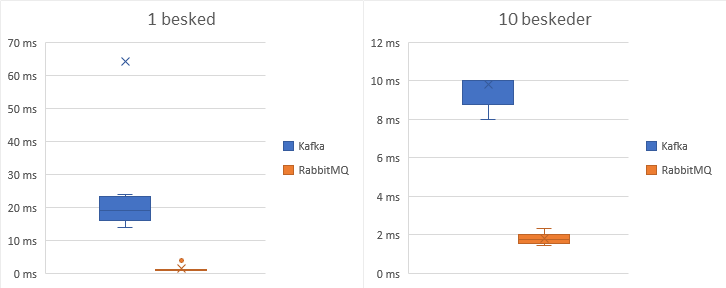
\includegraphics[width=5.5in,height=3in]{media/media/image1.png}

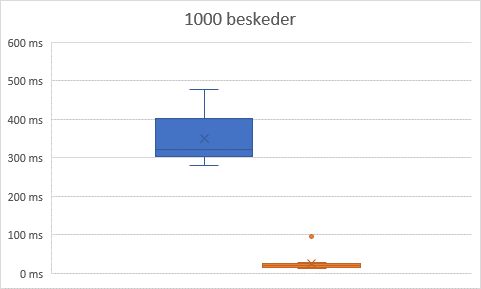
\includegraphics[width=5.5in,height=3in]{media/media/image2.png}

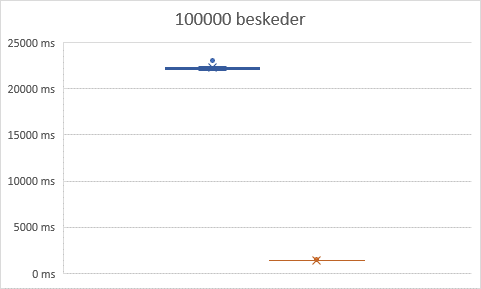
\includegraphics[width=5.5in,height=3in]{media/media/image3.png}


\hypertarget{fortolkninger-af-datasuxe6ttet.}{%
\subsection{Fortolkninger af
datasættet.}\label{fortolkninger-af-datasuxe6ttet.}}

Resultaterne viste overvejende stort at RabbitMQ var hurtigst til at
sende og modtage beskederne uafhængigt af det sendte antal. Dette
stemmer overens med at RabbitMQ skulle have lavere latency.\cite{kafka-rabbit-comparison}\\
På resultaterne kan man se at den største forskel sker når der sendes en
enkelt besked. Dette skyldes at den første besked der blev sendt med
Kafka, afveg meget fra de andre beskeders hastighed. Vi er ikke sikre på
årsagen, men formoder at Spring Boot Framework kunne være en faktor.
Efter 100 beskeder, virker det ikke til at antallet af beskeder har stor
forskel på latency

\hypertarget{fremtidigt-arbejde}{%
\subsection{Fremtidigt arbejde}\label{fremtidigt-arbejde}}

Det kunne være interessant at teste yderligere opsætninger af de to
teknologier.\\
Med stort nok throughput kunne det vise sig om Kafka, ville være
hurtigere end RabbitMQ.\\
Ligeledes kunne det være meget interessant at se hvordan teknologierne
ville præstere i større distribuerede systemer, men disse ting har vi
desværre ikke været i stand til at teste.

Kafka kunne blive testet med partitions for at se om det ville forbedre
ydeevnen, og med RabbitMQ kunne man teste med persistente
konfigurationer, for at se om hastighederne ville være tættere på
Kafkas.

\hypertarget{reproducere-benchmarks}{%
\subsection{Reproducere benchmarks}\label{reproducere-benchmarks}}

For at reproducere resultaterne, kan du klone de følgende repositories
og køre dem på din egen maskine.\\
\textbf{Obs. det kræver at hhv. RabbitMQ og Kafka er installeret og
kørende}\\
\href{https://github.com/SOFTBoiS/RabbitMQ_Test}{\underline{https://github.com/SOFTBoiS/RabbitMQ\_Test}}\\
\href{https://github.com/SOFTBoiS/Kafka-Producer-test}{\underline{https://github.com/SOFTBoiS/Kafka-Producer-test}}\\
\href{https://github.com/SOFTBoiS/Kafka-Consumer-test}{\underline{https://github.com/SOFTBoiS/Kafka-Consumer-test}}

\pagebreak
\hypertarget{konklusion}{%
\section{Konklusion}\label{konklusion}}

I vores research og test af de to teknologier er vi kommet frem til, at
der ikke er en af dem der direkte er bedst. De har hver deres styrker og
svagheder.\\
RabbitMQ virker dog som udgangspunkt det bedste valg i mange tilfælde.
Det er mere simpelt at bruge, og i vores tests har det lavere latency
end Kafka. Så hvis man som udgangspunkt har brug for en message broker,
mellem applikationer eller microservices, er RabbitMQ et rigtigt godt
bud.

Med RabbitMQ får man mulighed for at vælge mellem et større udvalg af
protokoller, og holder sig ligeledes mere åben til i fremtiden at kunne
skifte protokol, hvis man ønsker. Kafka er derimod låst fast i sin egen
version, som ikke kan udskiftes.

RabbitMQ er hurtigere til at sende og modtage beskeder. Kafka skulle dog
være bedre, når der skal sendes stort throughput, da RabbitMQ bliver
mindre effektivt i den situation.

RabbitMQ har i modsætning til Kafka routing og har mulighed for priority
queues, så hvis det er et krav, er RabbitMQ den rette teknologi. Kafka
er derimod bedre, hvis man skal persistere sit data, eller analysere
dataene mens den sendes.

Så overordnet set: Hvis man skal persistere eller genlæse sit data, og
har brug for at analysere dataene løbende eller skal streame store
mængder data, giver det mening at vælge Kafka.\\
Hvis ikke nogen af de ting gør sig gældende, bør man vælge RabbitMQ, da
det er mere simpelt, hurtigt og fleksibelt.
\pagebreak
\bibliography{references.bib}
\end{document}
